\documentclass[a4paper,12pt]{article}
\usepackage{amsmath,amsfonts,amsthm,amssymb, mathtools,steinmetz, gensymb, siunitx}	% LOADS USEFUL MATH STUFF
\usepackage{xcolor,graphicx}
\usepackage[a4paper]{geometry} 				% ADJUSTS PAGE
\usepackage{setspace}
\usepackage{physics}
\usepackage{caption}
\usepackage{tikz}
\usepackage{pgf,tikz,pgfplots}
\usepackage{mathrsfs}
\usepackage{amsbsy}
\usepackage{fancyhdr}
\usepackage{float}
\usepackage{array}
\usepackage{booktabs}
\usepackage{newpxtext}
\usepackage{unicode-math}
\usepackage{braket}
\setmathfont{Libertinus Math}

\usetikzlibrary{decorations.pathreplacing,decorations.markings}
\usepgfplotslibrary{fillbetween}

\newgeometry{left=1cm,top = 2.5cm, bottom = 1.75cm, right = 1cm}

\newcommand{\defeq}{:=}
\newcommand\block[1]{\hspace*{#1}}
\newcommand{\rpm}{\sbox0{$1$}\sbox2{$\scriptstyle\pm$}
	  \raise\dimexpr(\ht0-\ht2)/2\relax\box2 }
\newcommand{\af}{\pmb{\hat a_1}}
\newcommand{\as}{\pmb{\hat a_2}}
\newcommand{\at}{\pmb{\hat a_3}}
\newcommand\uv[1]{\pmb{\hat {#1}}}
\newcommand\vect[1]{\pmb{{#1}}}
\newcommand\dprod{\pmb{\cdot}}
	  
\pgfplotsset{compat=newest}
\newlength{\QNo}
\settowidth{\QNo}{2.}

\newlength{\QLetter}
\settowidth{\QLetter}{(a)}

\pagestyle{fancy}
\rhead{Quantum mechanics Problem Set}
\lhead{J. L. Gouws}


\begin{document}
\fontencoding{T1}
\fontfamily{ppl}\selectfont
{\Large \textbf{Quantum mechanics Assignment 1}} \hfill {\Large \textbf{J L Gouws}}\\
\block{1.0cm} {\large \textbf{\today}} \hfill {\large \textbf{26634554}}\\
\thispagestyle{empty}
\fontencoding{T1}

1.
\begin{minipage}[t]{0.9\textwidth}
  \begin{align*}
    \left(\bra{\psi} + \alpha* \bra{\phi}\right)\left(\alpha \ket{\phi} + \ket{\psi}\right)
  \end{align*}
\end{minipage}
$\phantom{1.}$
\begin{minipage}[t]{0.9\textwidth}
  c).
  \begin{minipage}[t]{\textwidth}
    The following vectors can be used as primitive translation vectors of a simple cubic lattice:
    \begin{equation*}
      \af = a \uv{x} \qquad \as = a \uv{y} \qquad \at = a \uv{z}
    \end{equation*}
    Which has the following reciprocal lattive basis vectors:
    \begin{equation*}
      \uv{b_1} = \frac{2 \pi}{a} \uv{x} \qquad \uv{b_2} = \frac{2 \pi}{a} \uv{y} \qquad \uv{b_3} =  \frac{2 \pi}{a}\uv{z}
    \end{equation*}
    Now for the plane $[hkl]$:
    \begin{align*}
                  & \pmb{G} = \frac{2 \pi h}{a} \uv{x} + \frac{2 \pi k}{a} \uv{y} + \frac{2 \pi l}{a} \uv{z}\\
      \Rightarrow & \left| \pmb{G} \right| = \sqrt{4 \pi^2 \frac{h^2 + k^2 + l^2}{a^2}}\\
      \Rightarrow & \left| \pmb{G} \right| = \frac{2 \pi}{a} \sqrt{h^2 + k^2 + l^2}
    \end{align*}
    Hence using the fromula for interplanar separation:
    \begin{align*}
                      & d_{hkl} = \frac{2 \pi}{\frac{2 \pi}{a} \sqrt{h^2 + k^2 + l^2}}\\
      \Leftrightarrow & d^2_{hkl} = \frac{a^2}{h^2 + k^2 + l^2}
    \end{align*}
  \end{minipage}
\end{minipage}
  \begin{figure}
  \centering
  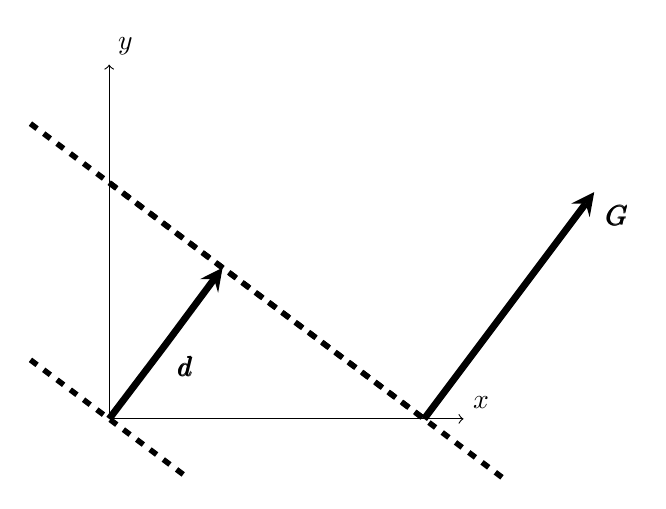
\begin{tikzpicture}
    \draw[->] (0, 0) -- (4.5, 0) node[anchor = south west] {$x$};
    \draw[->] (0, 0) -- (0, 4.5) node[anchor = south west] {$y$};
    \draw[dashed, line width = 2] (-1, 3.75) -- (5, -0.75);
    \draw[dashed, line width = 2] (-1, .75) -- (1, -0.75);
    \draw[dashed, line width = 2] (0, 3) -- (4, 0);
    \draw[->, line width = 2.5, >=stealth] (0, 0) --  (0.72, 0.95) node[anchor = north west] {$\pmb{d}$}-- (1.44, 1.92);
    \draw[->, line width = 2.5, >=stealth] (4, 0) -- (6.16, 2.88) node[anchor = north west] {$\pmb{G}$};
  \end{tikzpicture}
  \caption{The interplanar separation.}
  \label{fig:planeSep}
\end{figure}

\begin{figure}
  \centering
  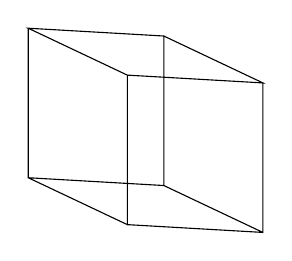
\begin{tikzpicture}
    \begin{axis}[
      axis x line=none,
      axis y line=none,
      axis z line=none,
      axis equal image,
%      view = {20}{30}
    ]
    \addplot3 [mark=none] coordinates 
    {
      (0, -1, 2)
      (3, 0, 2)
      (0, 1, 2)
      (-3, 0, 2)
      (0, -1, 2)
      (0, -1, -2)
      (3, 0, -2)
      (3, 0, 2)
      (3, 0, -2)
      (0, 1, -2)
      (0, 1, 2)
      (0, 1, -2)
      (-3, 0, -2)
      (-3, 0, 2)
      (-3, 0, -2)
      (0, -1, -2)
      (0, -1, 2)
      (0, -1, -2)
    };
    \end{axis}
  \end{tikzpicture}
  \caption{The first Brillouin zone of a hexagonal lattice}
  \label{fig:firsBrillouin}
\end{figure}

2.
\begin{minipage}[t]{0.9\textwidth}
  a).
  \begin{minipage}[t]{\textwidth}
    The volume of the primitive cell is given by:
    \begin{equation*}
      V = \af \dprod (\as \times \at)
    \end{equation*}
    We have:
    \begin{equation*}
      \as \times \at = - \sqrt{3}\frac{ac}{2} (- \uv{y}) + \frac{ac}{2} \uv{x} = \sqrt{3}\frac{ac}{2} \uv{y} + \frac{ac}{2} \uv{x}
    \end{equation*}
    Thus:
    \begin{equation*}
      V = \frac{\sqrt{3} a^2c}{4} + \frac{\sqrt{3} a^2c}{4} = \sqrt{3} \frac{a^2c}{2}
    \end{equation*}\\
  \end{minipage}
  b).
  \begin{minipage}[t]{\textwidth}
    We have by the definition of the reciprocal lattice vectors:
    \begin{equation*}
      \uv{b_1} = 2 \pi \frac{\as \times \at}{V} = \frac{2 \pi}{V}
      \left|
      \begin{matrix}
        \uv{x} & \uv{y} & \uv{z}\\
        -\frac{\sqrt{3}a}{2} & \frac{a}{2} & 0\\
        0 & 0 & c
      \end{matrix}
      \right|
      = \frac{2 \pi}{\sqrt{3}ac} \uv{x} + \frac{2\pi}{a}\uv{y}
    \end{equation*}
    \begin{equation*}
      \uv{b_2} = 2 \pi \frac{\at \times \af}{V} = \frac{2 \pi}{V}
      \left|
      \begin{matrix}
        \uv{x} & \uv{y} & \uv{z}\\
        0 & 0 & c\\
        \frac{\sqrt{3}a}{2} & \frac{a}{2} & 0
      \end{matrix}
      \right|
      =  - \frac{2 \pi}{\sqrt{3}ac} \uv{x} + \frac{2\pi}{a}\uv{y}
    \end{equation*}
    \begin{equation*}
      \uv{b_3} = 2 \pi \frac{\af \times \as}{V} = \frac{2 \pi}{V}
      \left|
      \begin{matrix}
        \uv{x} & \uv{y} & \uv{z}\\
         \frac{\sqrt{3}a}{2} & \frac{a}{2} & 0\\
        -\frac{\sqrt{3}a}{2} & \frac{a}{2} & 0
      \end{matrix}
      \right|
      = \frac{2 \pi}{V}\frac{\sqrt{3}a^2 - (-\sqrt{3}a^2)}{2}
      = \frac{2 \pi}{c} \uv{z}
    \end{equation*}
  \end{minipage}

  c).
  \begin{minipage}[t]{\textwidth}
    The first Brillouin zone is described by the planes that bisect the following vectors perpendicularly:
    \begin{gather*}
      \frac{2 \pi}{\sqrt{3}ac} \uv{x} + \frac{2\pi}{a}\uv{y}\\
      - \frac{2 \pi}{\sqrt{3}ac} \uv{x} - \frac{2\pi}{a}\uv{y}\\
      -\frac{2 \pi}{\sqrt{3}ac} \uv{x} + \frac{2\pi}{a}\uv{y}\\
      \frac{2 \pi}{\sqrt{3}ac} \uv{x} - \frac{2\pi}{a}\uv{y}\\
      \pm \frac{2 \pi}{c} \uv{z}\\
    \end{gather*}
    This can be seen in Fig.~\ref{fig:firsBrillouin},
    it is a rhombic prism.
  \end{minipage}
\end{minipage}
\end{document}
